\documentclass[10pt]{beamer}

\usepackage{amsmath,amssymb}
\usepackage{zxjatype}
\usepackage[ipa]{zxjafont}
\usetheme[progressbar=frametitle]{metropolis}
\usepackage{tikz}
\usepackage{tikzsymbols}
\usepackage{appendixnumberbeamer}
\usepackage{minted}
\usepackage{url}

\usetikzlibrary{positioning}
\usefonttheme[onlymath]{serif}

% --- page number ---
\setbeamertemplate{footline}{%
	\raisebox{10pt}{\makebox[\paperwidth]{\hfill\makebox[7em]{\normalsize\texttt{\insertframenumber/\inserttotalframenumber}}}}%
}

% --- title logo ---
\newcommand{\myinsertlogo}[1]{%
\begin{tikzpicture}[overlay, remember picture]
    \node[above left=1cm and .8cm of current page.south east] {\includegraphics[width=2.25cm]{#1}};
\end{tikzpicture}}

% --- utils ---
\newcommand{\mymain}[1]{\textcolor{mLightBrown}{#1}}
\newcommand{\myaccent}[1]{\textcolor{mLightGreen}{#1}}
\newcommand{\red}[1]{\textcolor{red}{#1}}
\newcommand{\blue}[1]{\textcolor{blue}{#1}}

\title{Introduction to OpenCV}
\date{\today}
\author{Satoshi Murashige}
\institute{Mathematical Informatics Lab., NAIST}

\begin{document}
	\begin{frame}[plain]
		\maketitle
		\myinsertlogo{naist.pdf}
	\end{frame}
	\begin{frame}{Text books}
		『詳解 OpenCV 3』
	\end{frame}
	\begin{frame}{Table of Contents}
		\begin{enumerate}
			\item 基本的な画像処理
				\begin{itemize}
					\item 1章:概要
					\item 2章:OpenCV入門
					\item 10章:フィルタとコンボリューション
				\end{itemize}
			\item 物体検出
				\begin{itemize}
					\item 12章:画像解析
					\item 13章:ヒストグラムとテンプレートマッチング
					\item 14章:輪郭
				\end{itemize}
			\item 動画解析
				\begin{itemize}
					\item 15章:背景除去
					\item 16章:キーポイントと記述子
					\item 17章:トラッキング
				\end{itemize}
			\item 3次元復元
				\begin{itemize}
					\item 18章:カメラモデルとキャリブレーション
					\item 19章:射影変換と3次元ビジョン
				\end{itemize}
		\end{enumerate}
	\end{frame}

	\begin{frame}{サンプルコードについて}
		\begin{itemize}
			\item テキスト中のプログラムはすべてC++で書かれている
			\item 今回使用するコードはそれらをPython向けに書き直したもの
				\begin{itemize}
					\item 全部は書き直していない \Winkey[1.5]
					\item なるべくPythonicなスタイルにするのと説明の都合により機能が異なることがある
				\end{itemize}
		\end{itemize}
	\end{frame}

	\begin{frame}{Pythonを使用するメリット・デメリット}
		\begin{itemize}
			\item Pythonを使用するメリット \red{\Smiley[1.5]}
				\begin{itemize}
					\item コンパイル不要なのでTry \& Errorがしやすい
					\item Python向けの強力な開発環境の恩恵を受けられる
					\item Pythonで書かれた他のモジュールとの組み合わせが容易になる
				\end{itemize}
			\item Pythonを使用するデメリット \blue{\Sadey[1.5]}
				\begin{itemize}
					\item 上手に書かないとめっちゃ遅くなる
					\item 上手に書いても最適化されたC++の速度には及ばない \\
						(リアルタイム性が求められるタスクでなければ最低限の最適化でOK)
				\end{itemize}
		\end{itemize}
	\end{frame}

	\begin{frame}[fragile]{前準備}
		\begin{itemize}
			\item サンプルコードのリポジトリをダウンロードする
				\begin{center}
					\url{https://github.com/eqs/opencv3-book-python.git}
				\end{center}
			\item 画像処理用の画像をダウンロードする
				\begin{itemize}
					\item \mymain{\texttt{cd}}コマンドで\mymain{\texttt{images}}に
						移動してから\mymain{\texttt{sh get\_images.sh}}を実行
				\end{itemize}
		\end{itemize}
	\end{frame}

	\section{1章:概要}

	\begin{frame}{title}
		aaa
	\end{frame}
	
	\section{2章:OpenCV入門}
	
	\begin{frame}[fragile]{初めてのプログラム--写真を表示する}

		\begin{minted}{python}
import cv2

img = cv2.imread('../images/color/Lenna.bmp')
assert img is not None, 'Loading image is failed.'

cv2.namedWindow('Example 2-1', cv2.WINDOW_AUTOSIZE)
cv2.imshow('Example 2-1', img)

cv2.waitKey(0)
cv2.destroyWindow('Example 2-1')
		\end{minted}
	\end{frame}
	
	\begin{frame}[fragile]{2つ目のプログラム--動画}
		動画やカメラの映像に対する処理を行う際は,
		このプログラムが雛型になる

		\scriptsize
		\begin{minted}{python}
import cv2

cv2.namedWindow('Example 2-3', cv2.WINDOW_AUTOSIZE)
cap = cv2.VideoCapture(0)
assert cap.isOpened(), 'Cannot open the video.'

while True:
    
    ok, frame = cap.read()

    if not ok:
        break
    
    cv2.imshow('Example 2-3', frame)
    
    key = cv2.waitKey(33)
    if key >= 0:
        break

cap.release()
cv2.destroyAllWindows()
		\end{minted}
	\end{frame}

	\begin{frame}[fragile]{OpenCVで画像を読み込み,Matplotlibで表示する:\\色チャネルの順番が逆になっているので注意}
		\scriptsize
		\begin{minted}{python}
import cv2
from matplotlib import pyplot as plt

img_bgr = cv2.imread('../images/color/Lenna.bmp')

assert img_bgr is not None, 'Loading image is failed.'
assert len(img_bgr.shape) == 3, 'Loaded image is not color'

# 画像をBGRからRGBに変換する
img_rgb = cv2.cvtColor(img_bgr, cv2.COLOR_BGR2RGB) 

# 変換前の画像を表示
plt.subplot(1, 2, 1), plt.imshow(img_bgr), plt.title('BGR image')
# 変換後の画像を表示
plt.subplot(1, 2, 2), plt.imshow(img_rgb), plt.title('RGB image')
plt.show()
		\end{minted}
	\end{frame}

	\begin{frame}{実行結果}
		OpenCVはカラー画像をBGR画像として読み込むが,
		MatplotlibはRGB画像として解釈しようとするので表示が変になる
		\begin{center}
			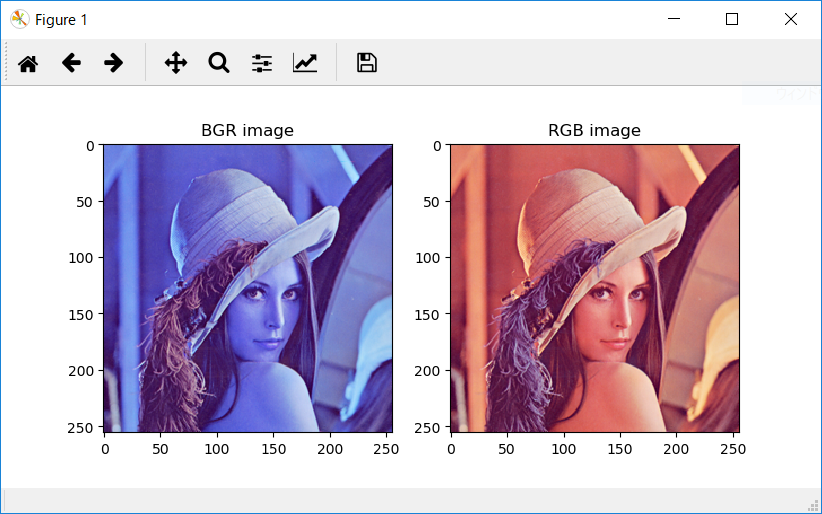
\includegraphics[width=10cm]{./figs/bgr_rgb.png}
		\end{center}
	\end{frame}
	
	\section{10章:フィルタとコンボリューション}
	
	\begin{frame}{画像フィルタリング}
		\begin{itemize}
			\item 画像を色の値からなる「2次元配列」ではなく,「2変数関数」と解釈する
			\item 画像フィルタリング:入力画像$I(x, y)$から新しい画像$I'(x, y)$を計算するアルゴリズム
				\begin{itemize}
					\item 例1:ある画像からぼけた画像を生成する
					\item 例2:ある画像を白と黒のみからなる画像に変換する
				\end{itemize}
		\end{itemize}
	\end{frame}
	
	\begin{frame}{画像フィルタリングの内容はカーネルによって定義される}
		\begin{itemize}
			\item 出力画像$I'(x, y)$の位置$(x, y)$における画素値は入力画像中の位置$(x, y)$周辺の画素から計算される
			\[ I'(x, y) = \sum_{i, j \in \mathit{kernel}} k_{i, j} \cdot I(x + i, y + j) \]
			\item 上式中の$k_{i, j}$を\mymain{線形カーネル(フィルタ)}と呼ぶ
			\item 画像に対してカーネル(線形,非線形問わず)を
				適用する操作を\mymain{コンボリューション}と呼ぶ
		\end{itemize}
	\end{frame}

	\begin{frame}{線形カーネルと適用のイメージ}
		\begin{center}
			\begin{tabular}{|c|c|c|}\hline
				$\frac{1}{9}$ & $\frac{1}{9}$ & $\frac{1}{9}$ \\ \hline
				$\frac{1}{9}$ & $\frac{1}{9}$ & $\frac{1}{9}$ \\ \hline
				$\frac{1}{9}$ & $\frac{1}{9}$ & $\frac{1}{9}$ \\ \hline
			\end{tabular}
		\end{center}
	\end{frame}

	\begin{frame}{線形カーネルによる画像フィルタリングの例:平滑化}

	\end{frame}
	
	\begin{frame}{境界の設定}
		
	\end{frame}
	
	\begin{frame}{閾値処理:ある値より上か下の画素を破棄する}
		
	\end{frame}
	
	\begin{frame}{大津の2値化}
		
	\end{frame}

\end{document}
